%
% Recomendaciones del NIST para la generación de llaves,
% capítulo de análisis y diseño para la generación de tokens.
% Proyecto Lovelace.
%

\capitulo{Generación de llaves}{sec:generacion_llaves}

% NIST 800-133 ---

\section{Conceptos clave}

\subsection{Métodos para la generación de llaves}
La generación de llaves se puede hacer por medio del uso de generadores de
bits aleatorios (\gls{gl:rbg}), de la derivación de llaves a partir de otras,
a partir de una contraseña; y del uso de un esquema de acuerdo entre llaves
(\textit{key agreement}); pero todas, de forma directa o indirecta, deben estar
basadas en la salida de un \gls{gl:rbg}.

\subsection{Dónde generar las llaves}
La generación de llaves criptográficas debe ir de acuerdo con el \gls{gl:fips}
140 (descrito en~\cite{nist_modulos_criptograficos}), y, si es necesario que
las llaves sean transferidas, se debe de hacer por medio de un canal seguro.
Además, todos los valores aleatorios requeridos para la generación de las
llaves deben ser generados dentro de un mismo módulo criptográfico.

\subsection{Fuerza de la seguridad}
La fuerza de la seguridad de un método es una medición de la complejidad
asociada a la recuperación de información secreta o de la seguridad relativa
a un algoritmo criptográfico a partir de datos conocidos.

Se dice que un método soporta la fuerza de seguridad, si la fuerza de
seguridad provista por dicho método es igual o mayor a la seguridad
requerida para la protección de la información.

\begin{itemize}
  \item La fuerza de seguridad para los \gls{gl:rbg} está basada en la
    \gls{gl:entropia} o aleatoriedad que provee el mismo \gls{gl:rbg}.

  \item La seguridad de un algoritmo criptográfico se basa en el hecho de
    que las llaves que usan fueron generadas por medio de procesos que las
    proveyeron de una \gls{gl:entropia} mayor o igual a la necesaria para el
    algoritmo, así como el mismo tamaño de las llaves.

  \item La fuerza de seguridad de una llave depende del algoritmo que la
    utilizará, su tamaño, el proceso con el que fue generada, y la forma en
    la que es utilizada.

\end{itemize}

\subsection{Usos de las salidas de los \gls{gl:rbg}}
Suponiendo que $K$ es una llave simétrica o un valor aleatorio que sirve
como entrada de un algoritmo generador de pares de llaves asimétricas, $K$
debe ser una cadena de bits tal que:

\begin{equation}
  \label{bits_K}
  K\: =\: U\: \oplus\: V
\end{equation}

Donde $U$ es una cadena de bits que se obtuvo de un \gls{gl:rbg} con el
soporte de la fuerza de seguridad requerida y $V$ es una cadena de bits de la
misma longitud, que además fue generada de manera tal que es independiente de
$U$ y viceversa. La independencia entre $U$ y $V$ se requiere debido a que se
tiene que evitar que el conocimiento de alguna de estas cadenas pueda usarse
para obtener información de la otra.

\subsection{Generación de pares de llaves asimétricas}
Los pares de llaves solo pueden ser generados o por el propietario del las
mismas llaves o por un tercero de confianza capaz de proveerlas.

Las llaves privadas deben permanecer secretas dentro del módulo criptográfico
del propietario o de un tercero de confianza; en caso de que se tengan que
transferir dichas llaves, se debe de garantizar que solo el propietario o la
parte generadora puedan verlas en claro.

\subsection{Generación de llaves simétricas}
Las llaves deben de ser generadas por una o varias de las entidades que
las compartirán, o por un tercero de confianza capaz de compartirlas de una
manera segura.

Las llaves que son generadas directamente de un \gls{gl:rbg} deben de cumplir
con la forma establecida en la ecuación~\ref{bits_K}.

Cuando sea necesario compartir una llave, su distribución debe de ser manual,
o por medio de un envolvimiento de la misma (\textit{key wrapping}), el cual
debe de soportar la fuerza de seguridad requerida para la protección de la
información que protege la llave.

Obtener llaves derivadas de una contraseña es una práctica cuestionable,
debido a que comúnmente la aleatoriedad en las contraseñas es mínima, por tal
razón, al generarse llaves de esta manera, es fuertemente recomendado que los
usuarios seleccionen contraseñas con una gran cantidad de \gls{gl:entropia}.
De cualquier manera, se considera que este tipo de llaves proveen una
\gls{gl:entropia} nula, a menos que la contraseña haya sido generada con
un \gls{gl:rbg}.

Cuando se tiene un conjunto de llaves $K_1, \dots, K_n$ generadas de forma
independiente, estas pueden ser combinadas entre sí para formar una llave $K$.
Igualmente, si se tiene un conjunto de bloques de información $V_1, \dots,
V_m$ que son independientes de sus respectivas llaves, se pueden combinar
estos bloques y sus llaves para formar otra llave.

Los métodos aprobados para generar llaves a partir de la combinación de
otras son:
\begin{itemize}

  \item La concatenación de varias llaves.
    $K\: =\: K_1\: \parallel\: \dots\: \parallel\: K_n$.

  \item La aplicación de compuertas \textit{xor} (o exclusiva) a varias llaves.
    $K\: =\: K_1\: \oplus\: \dots\: \oplus\: K_n$.

  \item La aplicación de compuertas \textit{xor} (o exclusiva) a varias llaves
    y bloques de información.
    $K\: =\: K_1\: \oplus\: \dots\: \oplus\: K_n\:
    \oplus\: V_1\: \oplus\: \dots\: \oplus\: V_m$.

\end{itemize}

Cuando sea necesario reemplazar una llave, la nueva llave debe de ser
completamente independiente de la anterior, para que el conocimiento de esta
última, no proporcione ningún conocimiento de la nueva.

% NIST 800-108 ---

\section{Funciones Pseudoaleatorias (PRF)}

Las funciones pseudoaleatorias o \gls{gl:prf} (ver sección
\ref{sec:generadores_pseudoaleatorios}) son funciones computables en
\gls{gl:tiempo_polinomial} con un índice o \gls{gl:semilla} $s$ y una variable
de entrada $x$, de manera que cuando $s$ se selecciona aleatoriamente de $S$,
es \gls{gl:computacionalmente_indistinguible} de una función aleatoria
definida en el mismo dominio y rango que $PRF(s,x)$.

Cuando una llave criptográfica $K_I$ es usada como la \gls{gl:semilla} de una
\gls{gl:prf}, su salida se puede utilizar como \gls{gl:material_de_llaves}.

Para la derivación de llaves se tiene permitido el uso del \gls{gl:hmac} o
del \gls{gl:cmac} como función pseudoaleatoria.

\section{Funciones de derivación de llaves (KDF)}

Las funciones de derivación de llaves o \gls{gl:kdf} son funciones que a
partir de una llave dada como entrada, pueden generar
\gls{gl:material_de_llaves} capaz de ser empleado por varios algoritmos
criptográficos.

Las llaves de entrada de este tipo de funciones son llamadas \textit{key
derivation keys} y deben ser llaves criptográficas generadas por medio de un
\gls{gl:rbg} o por un proceso automático de establecimiento de llaves.

El \gls{gl:material_de_llaves} segmentado es usado como un conjunto de llaves
criptográficas correspondientes a distintos algoritmos que pueden ofrecer
diferentes servicios, por lo tanto las \gls{gl:kdf} deben de definir una
manera de transformar este material en llaves distintas.

De forma general las \gls{gl:kdf} funcionan iterando $n$ veces una función
pseudoaleatoria para concatenar sus salidas hasta que se alcance la longitud
de bits deseada para el \gls{gl:material_de_llaves}.

\section{Modos de iteración}

Algo necesario para el funcionamiento de las \gls{gl:kdf} son los modos de
iteración, ya que definen las entradas que se tendrán y el orden de los campos
de salida en cada ciclo.

\subsection{Counter mode}
En la figura~\ref{diagrama_counter_mode} se aprecia la forma de operación de
este modo de iteración, en el que los datos de entrada son concatenados en una
cadena binaria de la forma: $Label \parallel 0x00 \parallel Context \parallel
{[L]}_2$ donde el $Label$ es un valor que identifica el propósito del
\gls{gl:material_de_llaves}, $0x00$ es un octeto de ceros, el $Context$ es una
cadena con la información relacionada al \gls{gl:material_de_llaves}, y
${[L]}_2$ es la longitud del \gls{gl:material_de_llaves} que se desea obtener
representada en binario. Como se observa, en este modo de iteración el
contador forma parte los datos de entrada de la \gls{gl:prf}.

\begin{figure}
  \begin{center}
    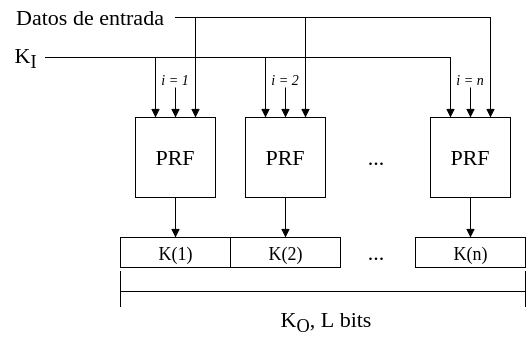
\includegraphics[width=0.75\linewidth]{diagramas/counter_mode}
    \caption{Diagrama del \textit{counter mode}.}
    \label{diagrama_counter_mode}
   \end{center}
\end{figure}

%Pseudocodigo excediéndose de los 80 para una correcta visualización el en pdf
\begin{pseudocodigo}[caption={Funcionamiento del \textit{counter mode}.},
label={mi:1}]
    entrada:   La llave $K_I$, la longitud $L$ y los valores de $Label$ y $Context$.
    salida:    $K_O$, con una longitud de $L$ bits.
    inicio
      calcular $n\: =\: [\frac{L}{h}]$, donde $h$ es la longitud de salida de la $PRF$.
      si $n$ > $2^r-1$, indicar error y parar; donde $r\: \leq\: 32$.
      $resultado(0) = \emptyset$
      para $i=1$ hasta $n$:
        $K(i)\: =\: PRF(K_I,\: {[i]}_2 \parallel Label \parallel 0x00 \parallel Context \parallel {[L]}_2 )$.
        $resultado(i)\: =\: resultado(i-1) \parallel K(i)$.
      $K_O =$ los L bits más a la izquierda del $resultado(n)$.
    fin
\end{pseudocodigo}

\subsection{Feedback mode}
Este modo de iteración opera tomando la salida de la \gls{gl:prf} en la
iteración anterior como parte los datos de entrada de la iteración actual.
Cabe resaltar que como se muestra en la figura~\ref{diagrama_feedback_mode},
es opcional tener un contador concatenado a estos datos, que son iguales que
en el modo de operación anterior, solo que con un
\gls{gl:vector_de_inicializacion} $IV$.

\begin{figure}
  \begin{center}
    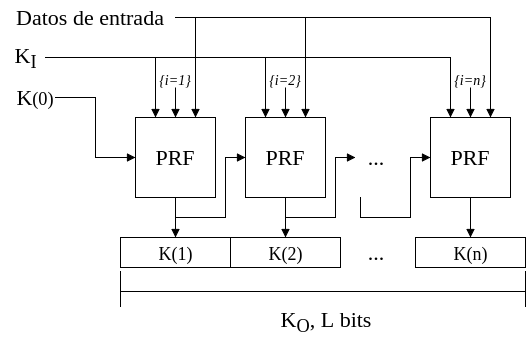
\includegraphics[width=0.75\linewidth]{diagramas/feedback_mode}
    \caption{Diagrama del \textit{feedback mode}.}
    \label{diagrama_feedback_mode}
   \end{center}
\end{figure}

%Pseudocodigo excediéndose de los 80 para una correcta visualización el en pdf
\begin{pseudocodigo}[caption={Funcionamiento del \textit{feedback mode}.},
label={mi:2}]
    entrada:   La llave $K_I$, la longitud $L$, el vector de inicialización IV
               y los valores de $Label$ y $Context$.
    salida:    $K_O$, con una longitud de $L$ bits.
    inicio
      calcular $n\: =\: [\frac{L}{h}]$, donde $h$ es la longitud de salida de la $PRF$.
      si $n$ > $2^{32}-1$, indicar error y parar.
      $resultado(0)\: =\: \emptyset$.
      $K(0) = IV$.
      para $i=1$ hasta $n$:
        $K(i)\: = \:PRF(K_I,\: K(i-1)\: \{\parallel {[i]}_2\}\: \parallel Label \parallel 0x00 \parallel Context \parallel {[L]}_2 )$.
        $resultado(i)\: =\: resultado(i-1) \parallel K(i)$.
      $K_O =$ los L bits más a la izquierda del $resultado(n)$.
    fin
\end{pseudocodigo}

\subsection{Double pipeline mode}
Como su nombre lo indica y a diferencia de los otros dos modos de iteración
mencionados, este usa dos flujos, donde un flujo es el encargado de generar
valores secretos, y el otro usa como entradas las salidas del primero para
obtener $K_O$. Los datos de entrada son iguales que en el primer modo de
iteración mencionado, y su funcionamiento está descrito en la figura
\ref{diagrama_dpipeline_mode}.

\begin{figure}
  \begin{center}
    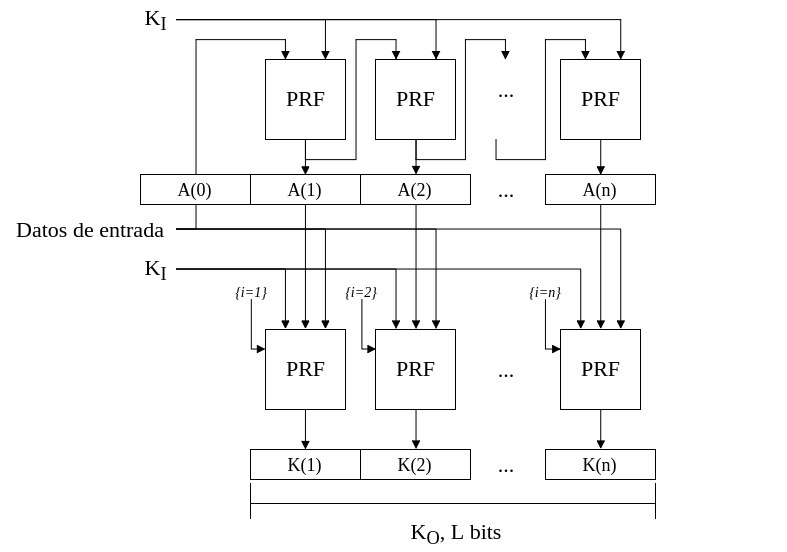
\includegraphics[width=0.75\linewidth]{diagramas/dpipeline_mode}
    \caption{Diagrama del \textit{double pipeline mode}.}
    \label{diagrama_dpipeline_mode}
   \end{center}
\end{figure}

%Pseudocodigo excediéndose de los 80 para una correcta visualización el en pdf
\begin{pseudocodigo}[caption={Funcionamiento del \textit{double pipeline mode}.},
label={mi:3}]
    entrada:   La llave $K_I$, la longitud $L$ y los valores de $Label$ y $Context$.
    salida:    $K_O$, con una longitud de $L$ bits.
    inicio
      calcular $n\: =\: [\frac{L}{h}]$, donde $h$ es la longitud de salida de la PRF.
      si $n$ > $2^{32}-1$, indicar error y parar.
      $resultado(0)\: =\: \emptyset$.
      $A(0)\: =\: IV\: =\: Label \parallel 0x00 \parallel Context \parallel {[L]}_2$
      para $i=1$ hasta $n$:
        $A(i)\: =\: PRF(K_I, A(i-1))$.
        $K(i)\: =\: PRF(K_I,\: A(i)\: \{\parallel {[i]}_2\}\: \parallel Label \parallel 0x00 \parallel Context \parallel {[L]}_2)$.
        $resultado(i) = resultado(i-1) \parallel K(i)$.
      $K_O =$ los L bits más a la izquierda del $resultado(n)$.
    fin
\end{pseudocodigo}

\subsection{Jerarquía de llaves}
El \gls{gl:material_de_llaves} proveniente de una derivación puede ser usado
una o más veces como llave de entrada de otras derivaciones subsecuentes, así,
es posible establecer una jerarquía en la que las llaves tienen distintos
niveles.

\section{Consideraciones de seguridad}

\subsection{Fuerza criptográfica}
La fuerza de seguridad de una \gls{gl:kdf} es medida por la cantidad de
trabajo requerido para distinguir su cadena de salida de una cadena de bits
que en verdad tenga una \gls{gl:distribucion_uniforme} y cuente con la misma
longitud, suponiendo que la llave de entrada $K_I$, es la única entrada
desconocida para la \gls{gl:kdf}.

\subsection{La longitud de la llave de entrada}
En algunas \gls{gl:kdf} el tamaño de la llave $K_I$ está definido por la
\gls{gl:prf} que usan internamente, por ejemplo cuando se usa el \gls{gl:cmac},
pero igualmente, otras \gls{gl:kdf} pueden usar llaves de cualquier tamaño,
como al usar el \gls{gl:hmac} como \gls{gl:prf}.

\subsection{Transformación de material de llaves a llaves criptográficas.}
La longitud en bits del \gls{gl:material_de_llaves} está limitada tanto por
el algoritmo relacionado a la salida de la \gls{gl:kdf}, como por el modo de
iteración que se usa.

\subsection{Codificación de los datos de entrada}
La información de entrada de una \gls{gl:kdf} consiste en diferentes campos
de datos, estos deben de estar ordenados de forma específica y sin ambigüedad,
de manera que se tenga un método de codificación capaz de mapear cada campo
individualmente. Esto es necesario para poder detectar ataques a la
\gls{gl:kdf} que dependan de la manipulación de esta información.

\subsection{Separación entre llaves}
Las llaves provenientes del \gls{gl:material_de_llaves} deben de estar
separadas criptográficamente, de tal manera que no se comprometa la seguridad
de ninguna de estas llaves derivadas. Cuando el \gls{gl:material_de_llaves}
se obtiene de múltiples ejecuciones de la \gls{gl:kdf} usando la misma llave
de entrada $K_I$, la \gls{gl:kdf} debe de garantizar que el
\gls{gl:material_de_llaves} de una ejecución no comprometa al de cualquier
otra.

\subsection{Enlace de contexto}
Todo el \gls{gl:material_de_llaves} debe estar ligado a todas las entidades
relacionadas para poder evitar errores de protocolo.
